In this section Bison is used to model the Ris\o~ AN3 power ramp fission gas release time series. More specifically, given the wide uncertainty in the input fission gas release parameters the problem of identifying parameter values resulting in Bison predictions most similar to experimental data is tackled. Since a single Bison simulation of the Ris\o~ AN3 power ramp is a computationally expensive, the surrogate construction techniques described in chapter \ref{chap:rom} will be employed. Recall that calibration exercises require thousands of instances of computer code simulations. Consequently, without the use of surrogates parameter calibration would not be feasible in this problem. Of the two surrogate construction techniques described, namely Kriging and the collocation approach, Kriging is more applicable for the problem in hand. Both surrogate techniques are designed for modeling surrogates of scalar quantities. However, in this problem a surrogate for an entire time series is desired. Of course, a surrogate can be constructed at each time-step but this would be extremely expensive considering there are $\mathcal{O}(100)$ time-steps. Kriging is used here mainly because it can most easily be extended when only a set and limited number of Bison simulations can be afforded. 

\subsection{Uncertain Parameters}
\label{subsec:uncertain_params}
In order to calibrate certain parameters it's necessary to first assign a valid range of values each parameter can potentially take on. In light of previous fission gas release parameter sensitivity research in \cite{Pastore2}, \cite{Swiler3}, and \cite{Johns} a total of eight parameters have been chosen for calibration in this research due to their propensity for influencing fission gas release behavior. The eight parameters are the initial fuel grain radius, fuel porosity, bubble surface tension, temperature, fuel grain radius, intra-granular gas atom diffusion coefficient, vacancy diffusion coefficient and resolution parameter. Each of the parameters is assumed to carry a uniform uncertainty distribution with lower and upper bounds estimated by Pastore et. al. \cite{Swiler3} \cite{Pastore2} using experimental values cited in published literature. The distributions are summarized in Table \ref{table:fgr_params}.
\begin{table} 
\caption{Fission gas release parameters used for calibration along with their uniform probability distributions.}
\label{table:fgr_params} 
\centering
\begin{tabular}{||c|c|c|c|c||} 
\hline \hline
\textbf{Description} & \textbf{Symbol} & \textbf{Lower Bound} & \textbf{Upper Bound} & \textbf{Scaled} \\ \hline
Initial Fuel Grain Radius & $r_{gr,0}$  & 2.0E-6 & 15.0E-6 & no \\ \hline
Fuel Porosity               & $P_f$      & 0.0      & 0.1      & no \\ \hline
Surface Tension           & $\gamma$  & 0.5     & 1.0      & no \\ \hline
Temperature               & $T$          & 0.95   & 1.05     & yes \\ \hline
Fuel Grain Radius         & $r_g$       & 0.4     & 1.6      & yes \\ \hline
Vacancy Diffusion Coef.  & $D_v$      & 0.1      & 10.0     & no \\ \hline
Resolution Parameter    & $b$         & 0.1      & 10.0     & no \\ \hline
Intra-granular Diffusion Coef. & $D_s$ & 0.316 & 3.162   & no \\ 
\hline \hline
\end{tabular}
\end{table}

The scaled column in Table \ref{table:fgr_params} denotes whether or not the parameter is scaled at each time-step in a Bison simulation, as described in Section \ref{sec:fgrTheory}. Temperature $T$ is a ubiquitous field parameter in Bison that gets passed into the \ac{SIFGRS} model, appearing most notably in Eq. \ref{eq:interal_gas_pressure} and \ref{eq:vacancy_change} along with the vacancy diffusion coefficient $D_v$. The bubble surface tension parameterizes how internal bubble gas pressure behaves and appears in Eq. \ref{eq:interal_gas_pressure}. The fuel grain radius appears in the grain boundary sweeping model \ref{eq:grain_boundary_sweeping} along with the equation describing the rate at which fission gases are released into the rod free volume in Eq. \ref{eq:fgr_rate_final}. In addition, the fuel grain radius $r_g$ is a boundary condition in the gas diffusion process in Eq. \ref{eq:bubble_diffusion}. The parameters $b$ and $D_s$ also appear in Eq. \ref{eq:bubble_diffusion}.   



\subsection{Principal Component Analysis}
\label{subsec:fgrPCA}
The problem at hand involves a time-dependent objective function, namely the fission gas release fraction throughout the course of a power ramp. Considering most surrogate methodologies, including the ones of interest in this thesis, are designed to handle single objective functions at a time, constructing a surrogate for an entire time series is problematic since a surrogate must be constructed at every time step. Such is especially the case when one does not know a priori whether or not a given time series will contain interesting features mid-cycle, such as jumps and peaks in the objective function. In addition, if pertinent experimental time series data is available and a calibration study is desired, a surrogate model for the entire time series will be necessary. Time dependency is not an issue if one is only interested in investigating, for example, beginning of life or end of life behavior. \ac{PCA} will be used in this thesis as a framework to create an efficient mapping between fission gas release parameters in \ac{SIFGRS} and the Ris\o~ AN3 power ramp fission gas release time series. 

\subsubsection{Theory}
 
As with many of the great ideas in linear algebra, the premise of \ac{PCA} rests on a change of basis. \ac{PCA} attempts to represent some original data samples in terms of a set of basis vectors that reduce redundancy and noise in the data. To this end, consider a matrix $\textbf{X}$ of $n$ observations and $k$ variables where the $k$ variables have been rescaled by their respective mean, as shown in Eq. \ref{eq:dataMatrix}. Rescaling by the mean will ensure that the projected data will live around the centroid of the new basis vectors.
\begin{equation}
\label{eq:dataMatrix}
 \textbf{X} =
  \begin{pmatrix}
   \vline & \vline & \cdots & \vline \\ 
   X_{1} & X_{2} & \cdots & X_{k} \\
   \vline & \vline & \cdots & \vline 
  \end{pmatrix}
\end{equation} 
The problem \ac{PCA} solves is that of choosing a set of expansion coefficients $\lbrace p_{1j}\rbrace_{j=1}^k$ such that,
\begin{equation}
\label{eq:pcaExpCoeffs}
 \textbf{Y}_{1} = \textbf{p}_{1}^{T}\textbf{X}^{T} = p_{11}X_{1} + p_{12}X_{2} + \cdots + p_{1k}X_{k}
\end{equation}
captures the largest variance in the data set. In other words, $\textbf{Y}_{1}$ will point in the direction of largest variance. To bound the potential values of $\textbf{p}_{1}$ the condition $\| \textbf{p}_{1} \|_2 = 1$ is enforced. Since it is unlikely that $\textbf{Y}_{1}$ will capture all the variance in the data, \ac{PCA} goes on to find $\textbf{Y}_{2}, ..., \textbf{Y}_{k}$ such that all the variance in the data is accounted for. Each $\textbf{Y}_{j}$ is independent from the other $\textbf{Y}_{i\not= j}$ to make sure there is no redundancy in capturing variance. Each $\textbf{Y}_{j}$ is referred to as the $j$-principal component. In matrix form, the workings of \ac{PCA} result in,
\begin{equation}
\label{eq:pcaRotation}
 \textbf{Y} = \textbf{P}^T\textbf{X}^T.
\end{equation}
From Eq. \ref{eq:pcaRotation} it becomes clear that the operator $\textbf{P}$ consisting of $\lbrace p_{ij}\rbrace_{i,j=1}^k$ has the effect of rotating the data in $\textbf{X}$ onto an uncorrelated set of axis. 

While the desired effect of operator $\textbf{P}$ to produce output $\textbf{Y}$ has been described, the question of how to find the expansion coefficients comprising $\textbf{P}$ remains. As described in \cite{Shlens}, the coefficients can be shown to be the loadings of the eigenvectors of the covariance matrix for $\textbf{X}$. The columns of $\textbf{P}$ are the eigenvectors of the symmetric matrix, 
\begin{equation}
\label{eq:covarMatrixPCA}
  \begin{pmatrix}
   \sigma_{1,1} & \sigma_{1,2} & \cdots & \sigma_{1,k} \\
                  & \sigma_{2,2} & \cdots & \sigma_{2,k} \\
                  &                 & \ddots & \vdots        \\
                  &                 &          & \sigma_{k,k}
  \end{pmatrix}
\end{equation}
where $\sigma_{i,j}$ represents the covariance between random variables $X_i$ and $X_j$. The eigenvalues of the matrix in Eq. \ref{eq:covarMatrixPCA} represent the amount of variance covered by the respective eigenvector. Before being placed into $\textbf{P}$, the eigenvectors should be sorted in descending order with respect to eigenvalue. 

The utility of \ac{PCA} lays in the fact that for most data sets the variance can be projected onto $\mathcal{O}(1)$ eigenvectors. To reveal this property the sorted eigenvalues can be plotted consecutively. \ac{PCA} can be viewed as a tool for reducing the dimensionality of a data set by opting to keep only the first $r$-principal components since a majority of the variance can be projected onto these components. Indeed, if only $r$ eigenvectors are kept then the projected data can written as,
\begin{equation}
\label{eq:projectedDataPCA}
 \textbf{Y}_r = \textbf{P}_r^T \textbf{X}^T.
\end{equation} 
Using Eq. \ref{eq:projectedDataPCA} the reduced-variance version of the data in $\textbf{X}$ can be reconstructed as,
\begin{equation}
\label{eq:reconstructedDataPCA}
 \textbf{X}_*^T = \textbf{P}_r \textbf{Y}_r
\end{equation} 
where it's noted that the inverse of a matrix with orthonormal columns is its transpose. The reconstructed data in Eq. \ref{eq:reconstructedDataPCA} represents perturbations around a centroid; the data mean must be added back in to obtain physical values. Using \ac{PCA} to express a data set in terms of a more meaningful and truncated basis allows one to filter out noise and identify structure in the data. Such possibilities allow one to glean insights into the main contributors of a data set's variance \cite{Bisgaard}.  

\subsubsection{Insights}

To obtain insight into the contributors of variance in Bison fission gas release time series, \ac{PCA} is applied to the data shown in Fig. \ref{fig:fgrSimulations}. Each of the 100 time series shown in Fig. \ref{fig:fgrSimulations} is induced by a different set of \ac{SIFGRS} parameters. Consequently, the time-stepping required for convergence in Bison varies from one time series to another. To perform \ac{PCA} on the data, fission gas release fractions must be compared at identical times throughout the 100 different samples. Consequently every power ramp time series output by Bison is interpolated using cubic splines and then sampled at 150 evenly spaced points. The covariance matrix central to \ac{PCA} in this case contains covariances between all 150 time steps. The eigenvalues of the covariance matrix are depicted in Fig. \ref{fig:fgrEvals}.
\begin{figure}
\caption{\label{fig:fgrEvals}
Cummulative variance carried by successive eigenvalues in the \ac{PCA} covariance matrix.}
 \begin{center}
  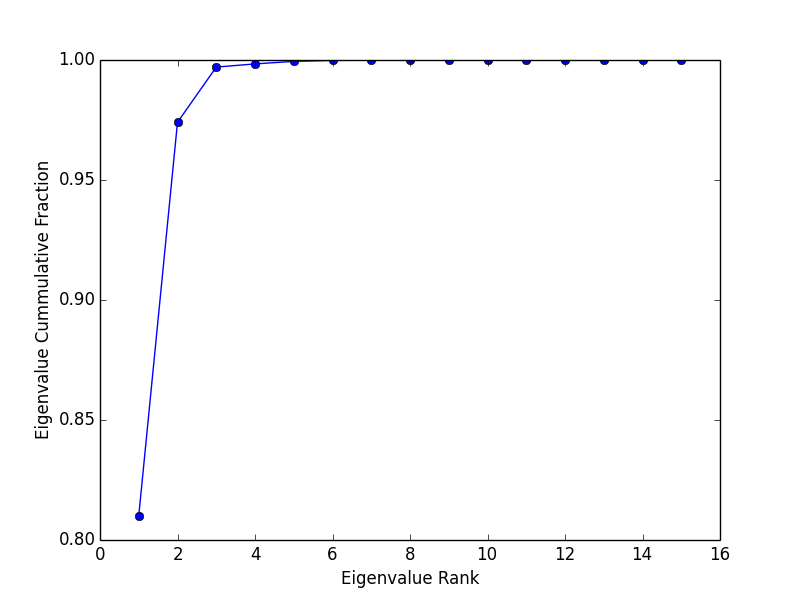
\includegraphics[scale=.75]{./Chapter4/fgr_evals.png}
 \end{center}
\end{figure}
As seen in Fig. \ref{fig:fgrEvals}, the three largest eigenvalues account for over 99\% of the variance. If the original time series data is rotated onto the corresponding three principal components using Eq. \ref{eq:projectedDataPCA}, each time series can be represented using only three expansion coefficients. Consequently, surrogates can be constructed for only the three expansion coefficients as a function of the \ac{SIFGRS} parameters. Instead of having to construct a surrogate at every time step, the principal component expansion coefficient surrogates act as a mapping to the entire time series.   

The three principal components corresponding to the three largest eigenvalues of the time series covariance matrix are plotted in Fig. \ref{fig:fgrEvecs}. The principal components enable insight into an underlying stochastic process by observing the magnitude of their coefficients \cite{Bisgaard}.  
\begin{figure}
\caption{\label{fig:fgrEvecs}
First three principal components of the time series covariance matrix.}
 \begin{center}
  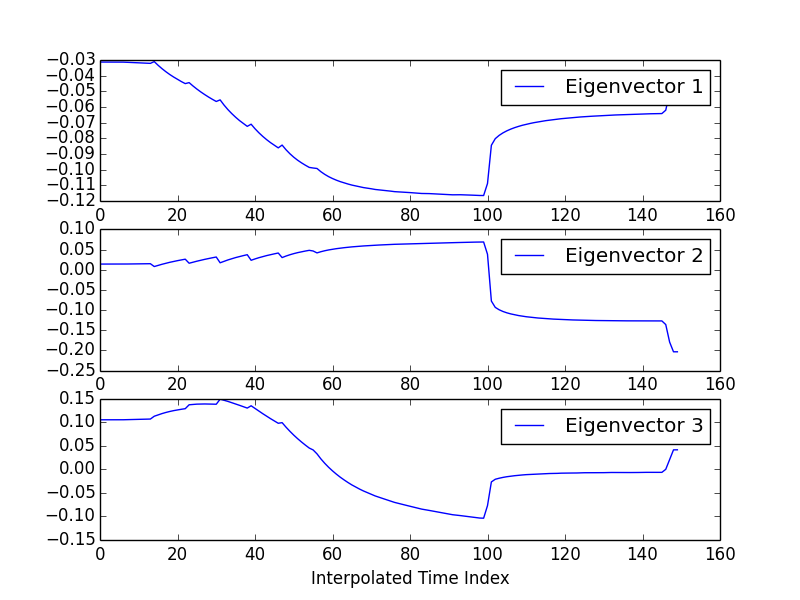
\includegraphics[scale=.75]{./Chapter4/fgr_evecs.png}
 \end{center}
\end{figure}
Each time index's magnitude in a principal component represents its influence on the component. From Fig. \ref{fig:fgrEvecs} it appears as though the first principal component is strongly influenced by the times in the middle of the power ramp, the second principal component is influenced by the times at the end of the power ramp and the third principal component is influenced most by the early stages of the power ramp. Further insights can be gleaned by plotting the principal components as time series and correlating the loadings with the \ac{LHS} values for the \ac{SIFGRS} parameters as in Fig. \ref{fig:principalCompTS}.     
\begin{figure}
\caption{\label{fig:principalCompTS}
Time series of the first principal component and correlations with \ac{SIFGRS} parameters.}
 \begin{center}
  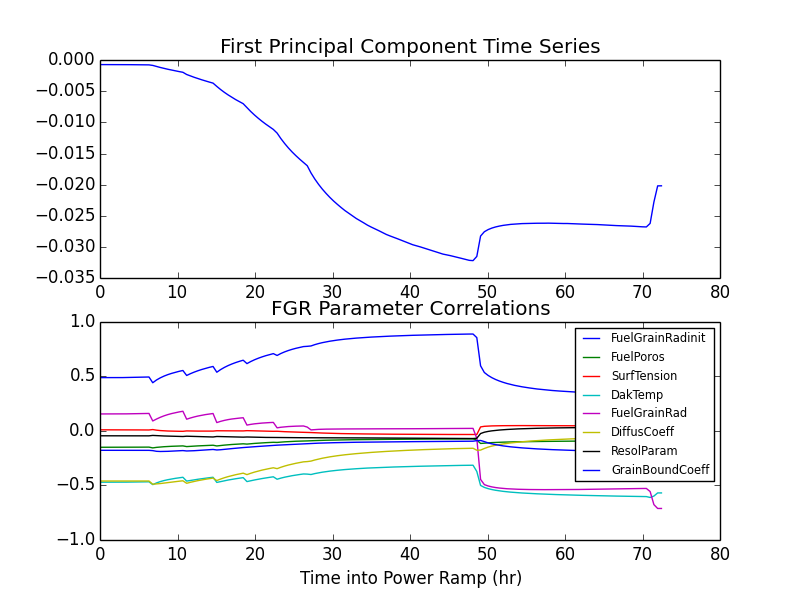
\includegraphics[scale=.75]{./Chapter4/firstPrincComp_FGR_Correlations.png}
 \end{center}
\end{figure}
The initial fuel grain radius appears to be the leading driver of the variance in the first principal component judging by its high correlation in the middle of the power ramp. Observe how in the late stages of the power ramp, the temperature and grain radius become primary contributors. 


\subsection{Time-Series Surrogate}
\label{subsec:ts_surrogate}
In Section \ref{subsec:fgrPCA} \ac{PCA} was used used to show that three eigenvectors are sufficient to capture over 99\% of the variance in Bison's simulated Ris\o~ AN3 power ramp fission gas release time series. The variation is caused by perturbations in the fission gas release parameters although they are not explicit in the \ac{PCA} framework. The Dakota code is used to create the 100 time series in the previous section. In accordance with each parameter's uniform distribution described in Table \ref{table:fgr_params}, Dakota made 100 sets of perturbations to the parameters using the \ac{LHS} method. Each of the 100 samples was then propagated through Bison and a time series of fission gas release was output. \ac{PCA} was then performed on the covariance matrix of the 100 samples. Consequently, there is a clear mapping from a set of eight fission gas release parameters to a time series. More specifically, there is a mapping from the i$^{th}$ set of eight parameters $R^{i}$ to the three expansion coefficients $\lbrace p_{i1}, p_{i2}, p_{i3} \rbrace$ that are capable of reproducing the time series, as described in Eq. \ref{eq:pcaExpCoeffs}. In order to predict new time series for a set of fission gas release parameters not in the set used to derive the three principal components this mapping must be generated. Kriging is used achieve the mapping.  

To start, using the Kriging description in Section \ref{sec:kriging} a surrogate is constructed for each of the expansion coefficients related to the three principal components responsible for over 99\% of the variance. Each of these surrogates $\hat{p}_{ij}$ for $j\in\left(1,2,3\right)$ accepts a set of fission gas release parameters and outputs a scalar expansion coefficient for the principal component $X_j$. In accordance with Eq. \ref{eq:pcaExpCoeffs} the predicted fission gas release time series is,
\begin{equation}
\label{eq:predicted_mean_fgr_ts}
 \hat{\mathcal{F}}^{i}(R^i) = \hat{p}_{i1}\left(R^i\right) X_1 + \hat{p}_{i2}\left(R^i\right) X_2 + \hat{p}_{i3}\left(R^i\right) X_3 + \mu  
\end{equation}
where $\mu$ is the mean release time series of the 100 simulations. Since Kriging surrogates return an uncertainty $\sigma_{\hat{p}_{ij}}$ along with a predicted scalar value, an uncertainty band can be derived for the time series in Eq. \ref{eq:predicted_mean_fgr_ts}.
\begin{equation}
\label{eq:predicted_std_fgr_ts}
 \sigma_{ \hat{\mathcal{F}}^i }^2 = \sigma_{\hat{p}_{i1}}^2 X_1^2 + \sigma_{\hat{p}_{i2}}^2 X_2^2 + \sigma_{\hat{p}_{i3}}^2 X_3^2 
\end{equation}
The shape of the uncertainty vector output by Eq. \ref{eq:predicted_std_fgr_ts} is equal to the number of time-steps utilized in the principal components. 

\subsubsection{Cross Validation}
\label{subsec:cross_validation}

With a Kriging formulation for predicting Ris\o~ AN3 power ramp fission gas release time series for any set of Bison fission gas release parameters in place, it is necessary to test the formulation. In other words, it's necessary to investigate the error in the formulation's predictions. If the Kriging surrogates can accurately predict their respective \ac{PCA} expansion coefficients then the formulation will be able to accurately predict gas release time series since Eq. \ref{eq:predicted_mean_fgr_ts} is just a linear combination of the predictions. To this end, a test set of 100 independent Bison simulations of the Ris\o~ AN3 power ramp were obtained. The simulations in the test set are completely isolated from those in the training set and not used in calculating the Kriging surrogates nor the principal components. There are several common approaches to judging the validity of a predictive model as described in \cite{Jones_Schonlau}. With training and test sets available at disposal are true expansion coefficient values, predicted values, and uncertainties in the predicted values. Using these components the standardized cross-validated residual is defined as,
\begin{equation}
\label{eq:stnd_xval_residual}
 \frac{ p_{ij} - \hat{p}_{ij} }{ \sigma_{\hat{p}_{ij}} } . 
\end{equation}  
The standardized cross-validated residuals for all three Kriging surrogates' predictions on the test set are shown in Fig. \ref{fig:xval_3sig_bands}. Note the Kriging models used to predict the expansion coefficients are built on 100 samples analyzed previously in Sec. \ref{subsec:fgrPCA}.  
\begin{figure}
\caption{\label{fig:xval_3sig_bands}
Cross validation of Kriging predictions for \ac{PCA} expansion coefficients using 3$\sigma$ band approach.}
 \begin{center}
  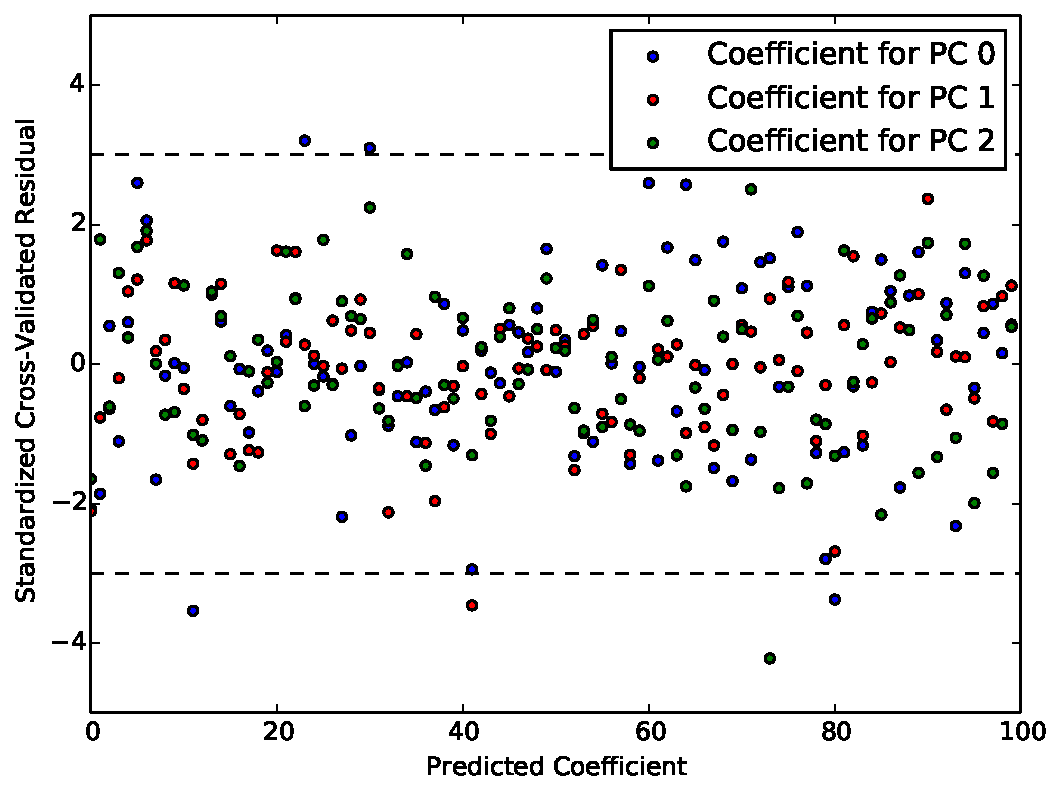
\includegraphics[scale=.75]{./Chapter4/xval_3sig_band.pdf}
 \end{center}
\end{figure}
Each point represents the number of standard deviations the true expansion coefficient is to the predicted coefficient. Some 99.7\% of points are expected to lie within the band $\left[-3, +3\right]$. Indeed, of the 300 points appearing in Fig. \ref{fig:xval_3sig_bands} some six lie outside the bands, which is a first indication that the predictive model has merit.  

In the second cross validation approach, the predicted values are plotted directly against the true values as shown in Fig. \ref{fig:xval_45degree}. Ideally, all points would lie on the 45$^{\circ}$ line, which would indicate that predictions perfectly match the true expansion coefficient values. The plots in Fig. \ref{fig:xval_45degree} show that the predicted values do generally approach this trend despite the presence of some noise. For predictions of each expansion coefficient in Fig. \ref{fig:xval_45degree} the results are plotted when 20, 60, and 100 random samples from the test set are utilized. Of course, less noise is present as the number of samples used to build the surrogates increase.  
\begin{figure}
\caption{\label{fig:xval_45degree}
Cross validation of Kriging predictions for \ac{PCA} expansion coefficients using 45$^\circ$ approach.}
 \begin{center}
  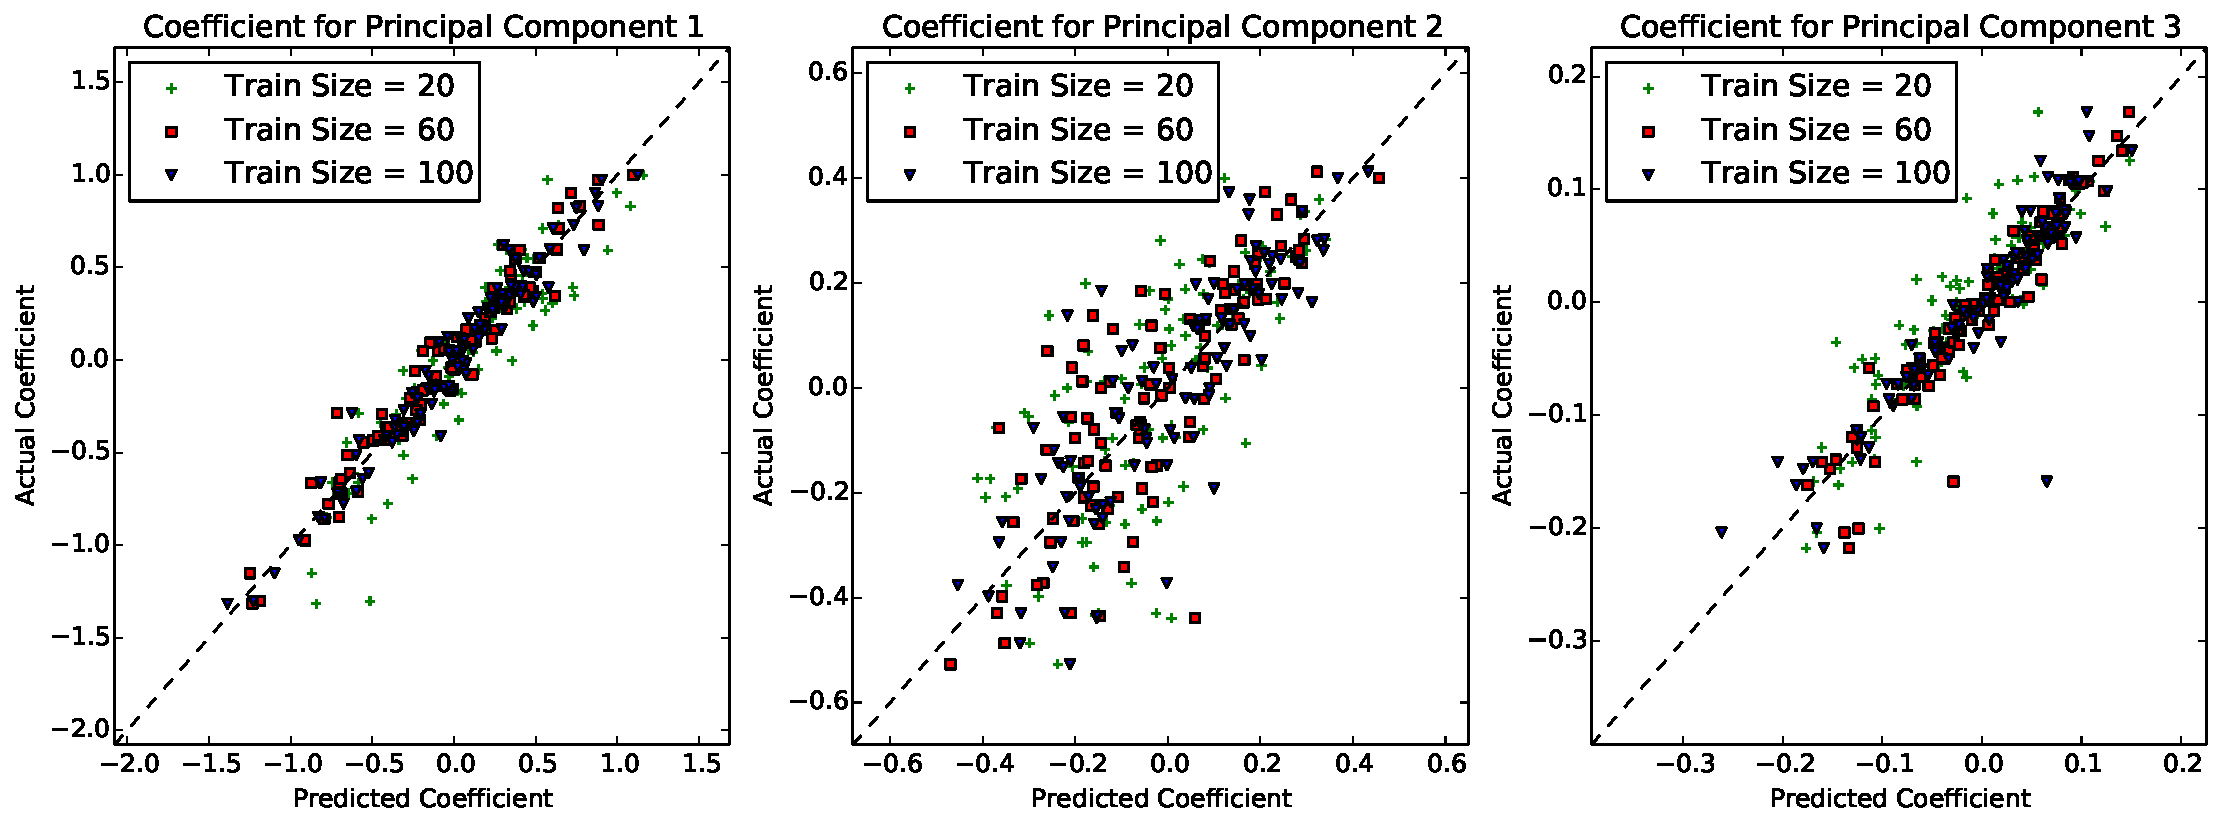
\includegraphics[scale=.4]{./Chapter4/xval_45degree.pdf}
 \end{center}
\end{figure}
Surprisingly, regardless of the training set size, predictions for the first principal component expansion coefficient are of the highest quality followed by the predictions for the expansion coefficients of the third principal component. It is most important to accurately predict expansion coefficients for the top principal components since they explain the most variance. Accurate prediction of lower principal components offers diminishing returns. Both inverse and logarithmic transforms were applied to the data as suggested in \cite{Jones_Schonlau} although no noticeable improvement was observed in prediction accuracy.   



